\chapter{TankUP - Desenvolvimento}
\label{chap:desen}

\section{Introdução}
\label{chap4:sec:intro}
Neste capítulo é feita uma exposição acerca dos elementos que constituem a aplicação, tal como a sua arquitetura de rede e a dinâmica entre as cenas utilizadas. É exemplificado e explicado o fluxo normal da aplicação, representando um jogo. \\ 
Devido a já terem sido abordadas as etapas nas quais eram incluídas utilizações de ferramentas externas, agora vai ser focado o que está por trás dos \textit{assets}, o que os controla e o que confere conteúdo à aplicação - os \emph{scripts} - formando os pilares do funcionamento de toda a estrutura formada pela conjunção das várias cenas construídas.

De maneira a uma melhor compreensão dos conteúdos apresentados a seguir, é importante ter em conta os seguintes termos: 
\begin{enumerate}
    \item \textit{Scene} - Aqui denominado como cena, é um conjunto de ecrãs da aplicação, sendo que estes ecrãs podem conter várias funcionalidades e gráficos, todos estes ligados através de \textit{scripts}.
    \item \textit{Script} - Agregação de código em \emph{C\#} que confere a capacidade de guardar e manipular informação a um objeto gráfico na cena. Pode estar associado a uma \textit{prefab}.
    \item \textit{Prefab} - Objeto complexo onde é guardada muita informação e funções, aproximando-se a uma classe "dinâmica", que pode interligar outras \textit{prefab}'s, cenas ou objetos. 
\end{enumerate}


\section{Constituição da aplicação}
\label{chap4:sec:TG}
De maneira a conseguir transmitir no que consistiu o processo de desenvolvimento da aplicação, é necessário descrever os seus dois constituintes mais importantes: a \emph{arquitetura de rede} - onde é explicado o funcionamento da comunicação entre os vários componentes de diferentes cenas entre objetos presentes em diferentes dispositivos, implicando comunicação através de rede - e a \emph{dinâmica entre cenas} - onde é demonstrado como é que o bom funcionamento da aplicação depende da interação entre vários objetos presentes em diferentes cenas. \\

De maneira a transmitir melhor a constituição da aplicação, procede-se agora à introdução do seu diagrama de classe \autoref{fig:diagrama}. Como pode ser visto neste, a aplicação é constituída por seis classes principais, que permitem o seu funcionamento. Em termos específicos, os seus propósitos são:
\begin{enumerate}
    \item \textbf{GameManager}: trata do menu na cena \emph{GameMenuScene} e, por isso, instancia e inicia o servidor e os clientes, garantindo depois que os clientes são conectados ao servidor.
    \item \textbf{Server}: aqui são definidos todos os métodos e variáveis que o servidor tem à sua disposição. O servidor vai esperar por ligações, vigiando um \textit{socket}. Quando um cliente se liga a este, vai transmitir a existência dessa ligação para todos os outros clientes e pode agora receber informação desse cliente, sendo essa informação constituída por mensagens codificadas de certa forma, de maneira a que cada uma corresponda a uma funcionalidade do servidor.
    \item \textbf{ServerClient}: quando os clientes são conectados ao servidor, este cria um \textit{ServerClient} para armazenar as informações do cliente, como o seu nome e o facto de este ser o \emph{host} ou não.
    \item \textbf{Client}: os clientes têm vários métodos associados como, por exemplo, a capacidade de enviar informação ao servidor, trabalhar com a informação que recebe do servidor ou criar e controlar um tabuleiro de jogo.
    \item \textbf{GameClient}: sempre que um cliente recebe informação de que um outro cliente também está conectado no servidor, este guarda a informação relativa a esse cliente.
    \item \textbf{MainBoardManager}: age como o controlador do tabuleiro, de maneira a controlar como e onde aparecem os \textit{assets} do jogo, usando também as interfaces do cliente que o criou para enviar directamente informação para o servidor a que o cliente que este está associado está ligado.
\end{enumerate}

\begin{figure}[!h]
    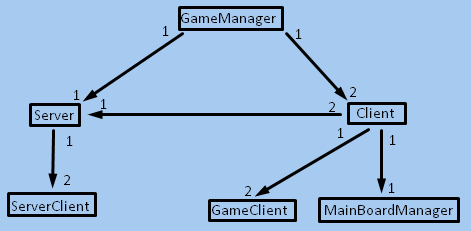
\includegraphics[width=8cm, height=5cm]{Screenshot_1.png}
    \centering
    \caption{Diagrama de classes.}
    \label{fig:diagrama}
\end{figure}

\subsection{Arquitetura de rede}
\label{chap4:subsec:rede}
A \textbf{arquitetura de rede} da aplicação consiste, muito basicamente, em dois clientes e um servidor, sendo que cada cliente tem um tabuleiro próprio e que a comunicação entre clientes é feita por meio do servidor. No entanto, há comunicação entre um cliente e o seu tabuleiro, assim como o tabuleiro consegue aceder a métodos próprios do cliente. 
Mais especificamente, existe uma cena de menu chamada \emph{GameSceneMenu}, onde é implementado um sistema de menu de maneira a que um utilizador possa iniciar um jogo (sendo um \emph{host}) ou juntar-se a um determinado jogo já existente (sendo um \emph{client}).  \\ 

Quando um jogador pressiona o botão \textit{host}, é instanciada uma \textit{prefab} de servidor com o endereço 127.0.0.1 e este é iniciado, ficando então à escuta de possíveis ligações. Também é instanciada uma \textit{prefab} de cliente, dado que o jogador que inicia o servidor também pode jogar, sendo este então conectado ao servidor. Se o jogador desejar conectar-se a um jogo que já foi criado (tendo conhecimento do endereço \ac{IP} local da máquina à qual se deseja conectar), este pode fazê-lo clicando no botão de \emph{Connect} e escrevendo o \ac{IP} da máquina do jogador com o qual este quer jogar.
Neste caso, é instanciada uma \textit{prefab} de cliente e ligada diretamente ao servidor designado pelo endereço \ac{IP} fornecido na caixa presente no menu de conexão do botão \emph{Connect}. \\ 

Quando o servidor é instanciado, este é também iniciado, o que significa que foi aberta uma \textit{socket} \ac{TCP} por onde é possível receber dados, e que o servidor está a escutar este \textit{socket} à procura de mais ligações de clientes.

Quando um cliente se liga ao servidor, este é inserido numa lista de clientes, sendo então registado no servidor com as suas informações básicas (como o seu nome e o facto de ser um \emph{host} ou não). Quando há dois clientes que se ligam a um dado servidor, este pára de escutar ligações novas dá início a uma sessão de jogo. Para fazer isto, o servidor passa as informações de cada cliente para uma lista de jogadores, de maneira a serem facilmente atingíveis. \\ 

A base da comunicação entre clientes e servidores são mensagens constituídas por conjuntos de caracteres, podendo estas gerar combinações que são depois interpretadas pelo destinatário, sendo ainda concatenadas com vária informação relativa ao remetente da mensagem. Desta forma, dependendo da mensagem recebida, diferentes ações vão ser tomadas por ambas as partes. \\ 

A comunicação servidor-cliente é assegurada por uma função de \emph{Broadcast} que envia um conjunto de caracteres para um ou mais objetos do tipo cliente. A comunicação cliente-servidor é, por sua vez, assegurada através da função \emph{Send}, que envia um conjunto de caracteres para o servidor ao qual o cliente se encontra ligado. 



\subsection{Dinâmica entre cenas}
\label{chap4:subsec:dinamica}
O jogo \emph{TankUP} é constituído por várias cenas, formando, em conjunto, todo o conteúdo do jogo que é apresentado ao jogador. Numa cena é tratado um determinado assunto pertinente para a etapa onde a aplicação se encontra num determinado momento, sendo que o tratamento de dados e o \textit{feedback} gráfico da aplicação é dependente dos objetos que estão presentes na presente cena. \\ 
De maneira a manter certa informação entre mudanças de cena, tal como o estado do jogo ou informações dos jogadores conectados ao servidor, é necessário não destruir os dados de determinados elementos da cena anterior. Bons exemplos destes casos são a permanência dos dados relativos ao servidor e aos clientes desde a cena em que são criados até ao final do ciclo de jogo, onde são então destruídos.

Por ordem de aparecimento, as cenas e o seu objectivo geral são:

\begin{table}[!h]
\centering
\caption{Informação acerca das cenas, ordenada por ordem de aparecimento.}

\label{tab:tabela_informacao_cenas}
\begin{tabular}{|c||l|l|}
\hline
\textbf{\#} & \textbf{Nome da cena} & \textbf{Objectivo geral da cena} \\
\hline
\hline
1 & Preloader & Carregamento inicial dos \textit{assets} do jogo \\
\hline	
2 & MenuScene & Menu inicial do jogo \\
\hline
3 & GameMenuScene  & Menu de conexão. Cria servidores e clientes\\
\hline
4 & Board & Tabuleiro onde decorre todo o jogo \\
\hline
\end{tabular}
\end{table}

A informação mais importante da aplicação é criada na cena \emph{GameMenuScene} - Instanciados os clientes e o servidor - e manipulada na cena \emph{Board} - comunicação entre servidor-cliente e cliente-tabuleiro.
A divisão da aplicação nas cenas supramencionadas garante que a sua modularidade, o que permite uma maior facilidade na execução de mudanças ao jogo e à sua manutenção.


\section{Fluxo da aplicação}
\label{chap4:sec:flow}
Nesta secção vai ser representada uma execução normal de um jogo.

\begin{enumerate}
    \item Ambos os jogadores iniciam a aplicação.
    \item Ambos os jogadores clicam o botão \textit{Play} na cena \emph{MenuScene} (\autoref{fig:screen1}).
    \item Ambos os jogadores chegam à cena \emph{GameMenuScene} (\autoref{fig:screen2}).
    \item Um jogador clica o botão de \emph{host} (jogador 1) (\autoref{fig:screen3}) e outro o botão de \emph{connect} (jogador 2) (\autoref{fig:screen4}).
    \item  No jogador 1 é criada uma instância de um servidor, o qual é iniciado, e uma instância de um cliente, a qual é ligada ao servidor criado. No jogador 2 é criada uma instância de um cliente, a qual é ligada ao servidor criado no jogador 1.
    \item Servidor recebe e aceita os pedidos dos jogadores, guardando a informação relativa a cada um. Dado haver dois jogadores conectados em simultâneo, o servidor informa os clientes de que podem mudar para a cena \emph{Board} (\autoref{fig:screen5}), começando o jogo.
    \item No início do jogo, os dois jogadores colocam os seus veículos na posição que desejarem, dentro da sua grelha. No final das colocações, os clientes passam a informação dos tabuleiros construídos ao servidor (\autoref{fig:screen6}).
    \item Quando o servidor recebe a informação dos tabuleiros de cada jogador, este envia uma informação ao jogador 1, com a informação acerca do tabuleiro do jogador 2, e dá-lhe permissão para clicar no botão de ataque. O jogador 2 está à espera.

    \item Quando o jogador 1 clica no tabuleiro, são apresentadas as jogadas anteriores que este fez, onde uma cruz vermelha significa um ataque falhado e um sinal de certo verde indica um ataque com sucesso (\autoref{fig:screen7}). No próximo clique do jogador no tabuleiro, é utilizada essa posição para efetuar um ataque ao jogador 2. O jogador 2 está à espera enquanto isto acontece. 
    \item Depois de escolhido o ataque, este é validado e enviado ao servidor se respeitar as regras do jogo. É então revogada a permissão do jogador 1 poder atacar e esta é dada ao jogador 2. Quando isto acontece, o seu tabuleiro é desenhado outra vez, de maneira a refletir o ataque que sofreu, com uma cruz vermelha na posição atacada (\autoref{fig:screen8}). O jogador 1 está à espera.
    \item Este ciclo de ataque e espera é repetido até que um dos jogadores consiga destruir todos os veículos inimigos, sendo então mostrada uma mensagem a ambos os jogadores com o vencedor.
    \item Jogo termina e ambos os jogadores são reencaminhados para a cena \emph{GameMenuScene}. 
\end{enumerate}
 
 \begin{figure}[!h]
    
\includegraphics[width=10cm, height=8cm]{sceen1.png}
    \centering
    \caption{Cena MenuScene}
    \label{fig:screen1}
\end{figure}

\begin{figure}[!h]
    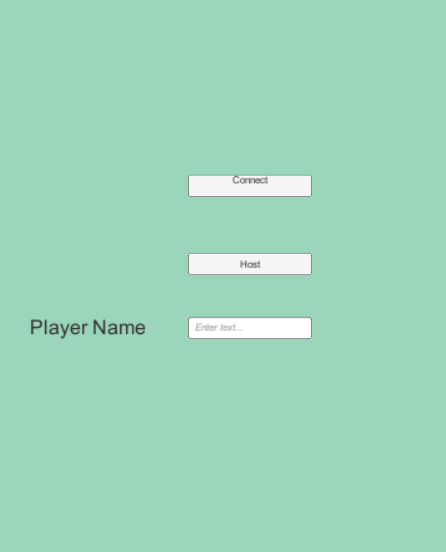
\includegraphics[width=10cm, height=8cm]{screen2.png}
    \centering
    \caption{Cena GameMenuScene}
    \label{fig:screen2}
\end{figure}

\begin{figure}[!h]
    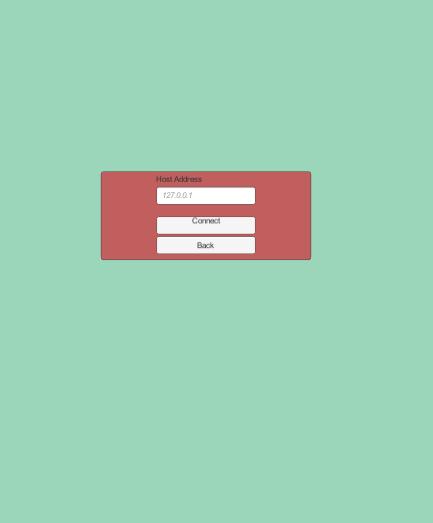
\includegraphics[width=10cm, height=8cm]{screen3.png}
    \centering
    \caption{GameMenuScene com seleção de host.}
    \label{fig:screen3}
\end{figure}

\begin{figure}[!h]
    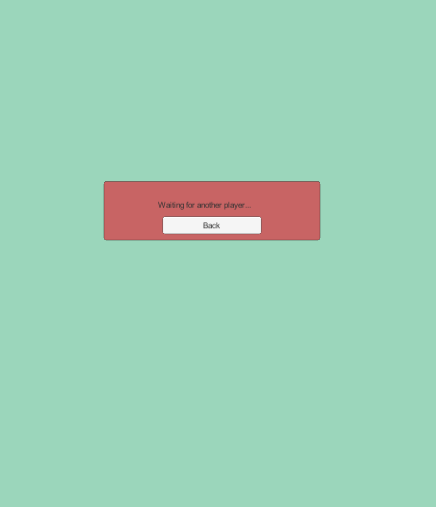
\includegraphics[width=10cm, height=8cm]{screen4.png}
    \centering
    \caption{GameMenuScene com seleção de conexão.}
    \label{fig:screen4}
\end{figure}
    
\begin{figure}[!h]
    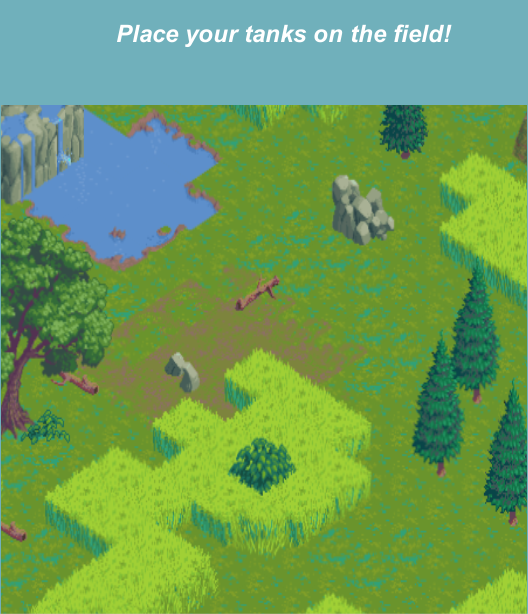
\includegraphics[width=10cm, height=8cm]{screen6.png}
% * <individuoamaral@gmail.com> 17:26:12 07 Jul 2017 UTC+0100:
% ALTERAR IMAGEM
    \centering
    \caption{Cena Board.}
    \label{fig:screen5}
\end{figure}
    
\begin{figure}[!h]
    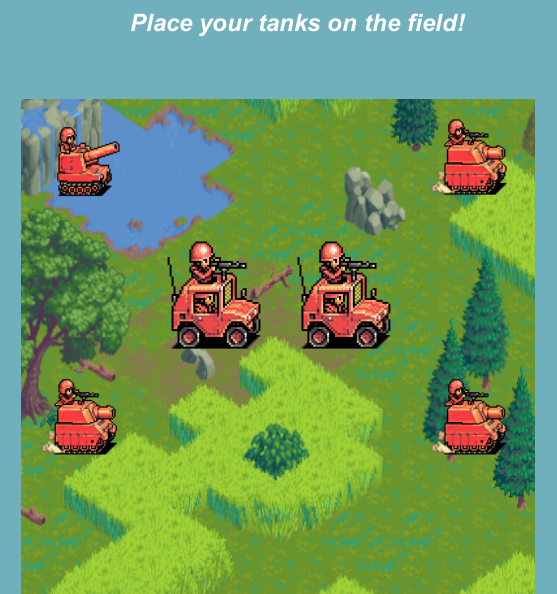
\includegraphics[width=10cm, height=8cm]{screen5.png}
    \centering
    \caption{Cena Board com veículos colocados.}
    \label{fig:screen6}
\end{figure}

\begin{figure}[!h]
    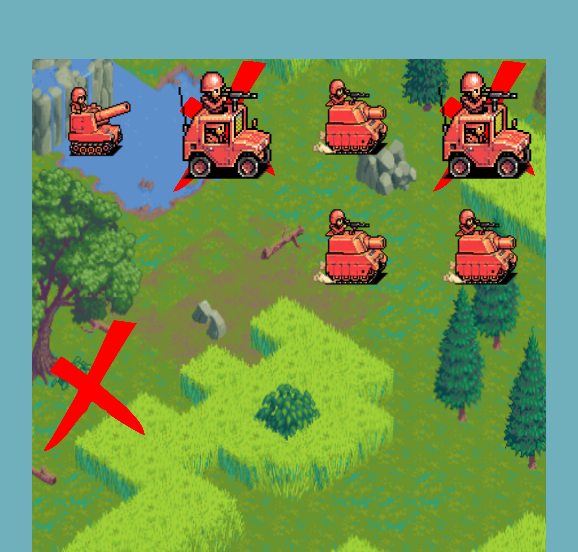
\includegraphics[width=10cm, height=8cm]{screen7.png}
    \centering
    \caption{Cena Board com ataques efectuados.}
    \label{fig:screen7}
\end{figure}

\begin{figure}[!h]
    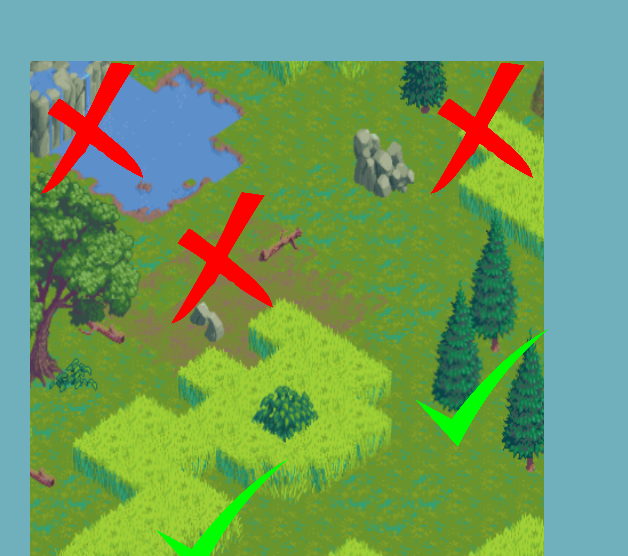
\includegraphics[width=10cm, height=8cm]{screen8.png}
    \centering
    \caption{Cena Board com veículos colocados e ataques sofridos.}
    \label{fig:screen8}
\end{figure}
    
\clearpage
Assim termina uma partida de \emph{TankUP}.

Em termos da integração do jogo na plataforma \emph{Android}, houveram algumas dificuldades de compatibilidade, devido a definições de \textit{build} erradas. Para ajudar na integração, assim como no \textit{playback} dos vídeos feitos no \emph{Blender}, usou-se o manual de referência do \emph{Android} [9].

\section{Conclusão}
\label{chap4:sec:conc}
Neste capítulo foram transmitidas as características dos constituintes mais importantes da aplicação: a \emph{arquitetura de rede} \autoref{chap4:subsec:rede} - criados dois clientes e um servidor, que vai estar a escutar uma \textit{socket} à procura de novas ligações de clientes, sendo que os dois clientes vão ser ligados a este, possibilitando assim comunicação servidor-cliente - e a \emph{Dinâmica entre cenas} \autoref{chap4:subsec:dinamica} - são criados vários objetos em diferentes cenas que têm de ser mantidos de maneira a não perder qualquer informação importante gerada numa cena passada. Com este entendimento acerca deles, é possível acompanhar um desenvolvimento de uma partida de \emph{TankUP}, como a que foi representada em \autoref{chap4:sec:flow}, estando assim completo o ciclo de vida da aplicação e, por isso, o ciclo de desenvolvimento de conteúdo. \\

A seguir, serão referidos trabalhos futuros, assim como melhorias que poderiam ser implementadas na aplicação de maneira a aumentar a sua qualidade. É também feita uma conclusão para as temáticas abordadas neste relatório e, por isso, na aplicação.